\vspace{0.2cm}
\noindent
This immediately connects the tensors to \emph{multivariate polynomials}. The scalar map
\[
f(\xb^{(1)},\dots,\xb^{(N)})=\sum_{i_1,\dots,i_N}\Tt_{i_1\cdots i_N}\,\xb^{(1)}_{i_1}\cdots \xb^{(N)}_{i_N},
\]
is a polynomial in the entries of the vectors and is \emph{multi-linear}: every variable appears with degree at most one (when viewed in each block of variables $\xb^{(k)}$). In the important special case where all inputs are the \emph{same} vector $\xb\in\RR^{d}$ and $\Tt\in\RR^{d\times\cdots\times d}$ has $N$ modes, the  contraction
\[
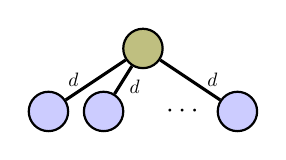
\begin{tikzpicture}[baseline=2ex]
    \tikzset{tensor/.style = {minimum size = 0.5cm,shape = circle,thick,draw=black,inner sep = 0pt},
             edge/.style   = {thick,line width=.4mm},
             every loop/.style={}}
    \def\x{0}\def\y{0}

    \node[tensor,fill=green!50!red!50!white] (T) at (\x,\y+0.8){$\Tt$};

    \node[tensor,fill=blue!20!white] (a) at (\x-1.2,\y){$\xb$};
    \node[tensor,fill=blue!20!white] (b) at (\x-0.5,\y){$\xb$};
    \node[draw=none] (dots) at (\x+0.5,\y){$\cdots$};
    \node[tensor,fill=blue!20!white] (z) at (\x+1.2,\y){$\xb$};

    \draw[edge] (T) -- (a) node [midway,left]{\scalebox{0.7}{\dimcolor{$d\ $}}};
    \draw[edge] (T) -- (b) node [near end,right]{\scalebox{0.7}{\dimcolor{$d$}}};
    \draw[edge] (T) -- (z) node [midway,right]{\scalebox{0.7}{\dimcolor{$\ d$}}};
\end{tikzpicture}
= \Tt \ttm{1}\xb \ttm{2}\xb \cdots \ttm{N}\xb
=
\sum_{i_1,\dots,i_N}\Tt_{i_1\cdots i_N}\,\xb_{i_1}\cdots \xb_{i_N} \in \RR.
\]
is a \emph{homogeneous} multivariate polynomial of degree $N$ (every monomial has total degree exactly $N$). The tensor entries are precisely the coefficients of this polynomial in the monomial basis $(\xb_{i_1}\cdots \xb_{i_N})_{i_1,\cdots,i_N}$.

If instead we contract an order-$(N+1)$ tensor $\Tt\in\RR^{ d\times\cdots\times d \times p}$ with $N$ copies of $\xb\in\RR^d$, leaving the last leg free, we obtain a vector-valued homogeneous polynomial map $\RR^d\to\RR^m$:
\[
p(\xb) = \Tt \ttm{1}\xb \ttm{2}\xb\cdots \ttm{N}\xb \in\RR^{p}.
\]

\vspace{0.2cm}
\noindent
Finally, \emph{non-homogeneous} polynomials can be obtained using a simple trick: \emph{append a constant $1$ to the input vector}. Let $\xb\in\RR^d$ and define the augmented vector $\tilde{\xb} =\begin{bmatrix}\xb\\1\end{bmatrix}\in\RR^{d+1}$. If $\widetilde{\Tt}\in\RR^{(d+1)\times\cdots\times(d+1)}$ is an order-$N$ tensor, then
\[
\tilde{p}(\xb)
:=
\widetilde{\Tt} \ttm{1}\tilde{\xb}\ttm{2}\tilde{\xb}\cdots\ttm{N}\tilde{\xb},
\]
is a polynomial in $\xb$ of degree at most $N$ (some factors can pick the last coordinate, which is the constant $1$, thereby lowering the degree of the corresponding monomials). In other words, a single homogeneous tensor polynomial in the augmented variables $(x_1,\dots,x_d,1)$ compactly represents a general multivariate polynomial in $(x_1,\dots,x_d)$. This viewpoint is especially useful in practice: it lets us treat bias terms and lower-degree interactions using the same contraction machinery as the homogeneous case, simply by adding one extra dimension to each mode and fixing it to $1$.  
